
\section{细化功能需求}
\begin{itemize}
    \item 教师信息、学生信息、课程信息自动导入数据库,且需要检查相应冲突(时间/地点/任课老师等)。
    \item 课程:一周内可能多次开课、可能通过论文考试、课时按照小时为单位。
    \item 共有三类权限人员:学生、老师、管理员(院系)。
    \item 三类权限人员使用各自登陆方式登陆系统后,可查看其各自权限下的所有信息。
    \item 学生权限:使用学号和密码登陆,查看成绩/课程表/选课申请。
    \item 老师权限:使用工号和密码登陆,查看课程花名册/管理选课事务申请。
    \item 管理员权限:使用root和密码登陆,查看所有信息并且自动导入/课程删除操作。
    \item 学生的选课和退课操作可以在任何时间进行,先到先得。
    \item 选课需要系统进行冲突检查(考试和上课)。
    \item 进行数据的本地化操作 或 在启动系统时有默认内部数据。
    \item 当且仅当课程的选课人数到达上限,学生可以填写选课申请。
    \item 相应课程的教师负责处理选课申请,可以选择通过或不通过。
    \item 当学生所选课程的选课人数超出教室可容纳人数时,系统自动驳回尚未处理的选课申请,关闭该课程的申请窗口。
    \item 学生可以查看选课申请状态。
    \item 学生不能申请已选课程。
    \item 考试时间为特定周到第18周,和上课时间不会冲突。
    \item 系统自动/手动导入学生课程成绩
    \item 学生可以查看该学期成绩单和总绩点
    \item 教师可以通过excel方式登分。
\end{itemize}


\begin{figure}[h]
    \centering
    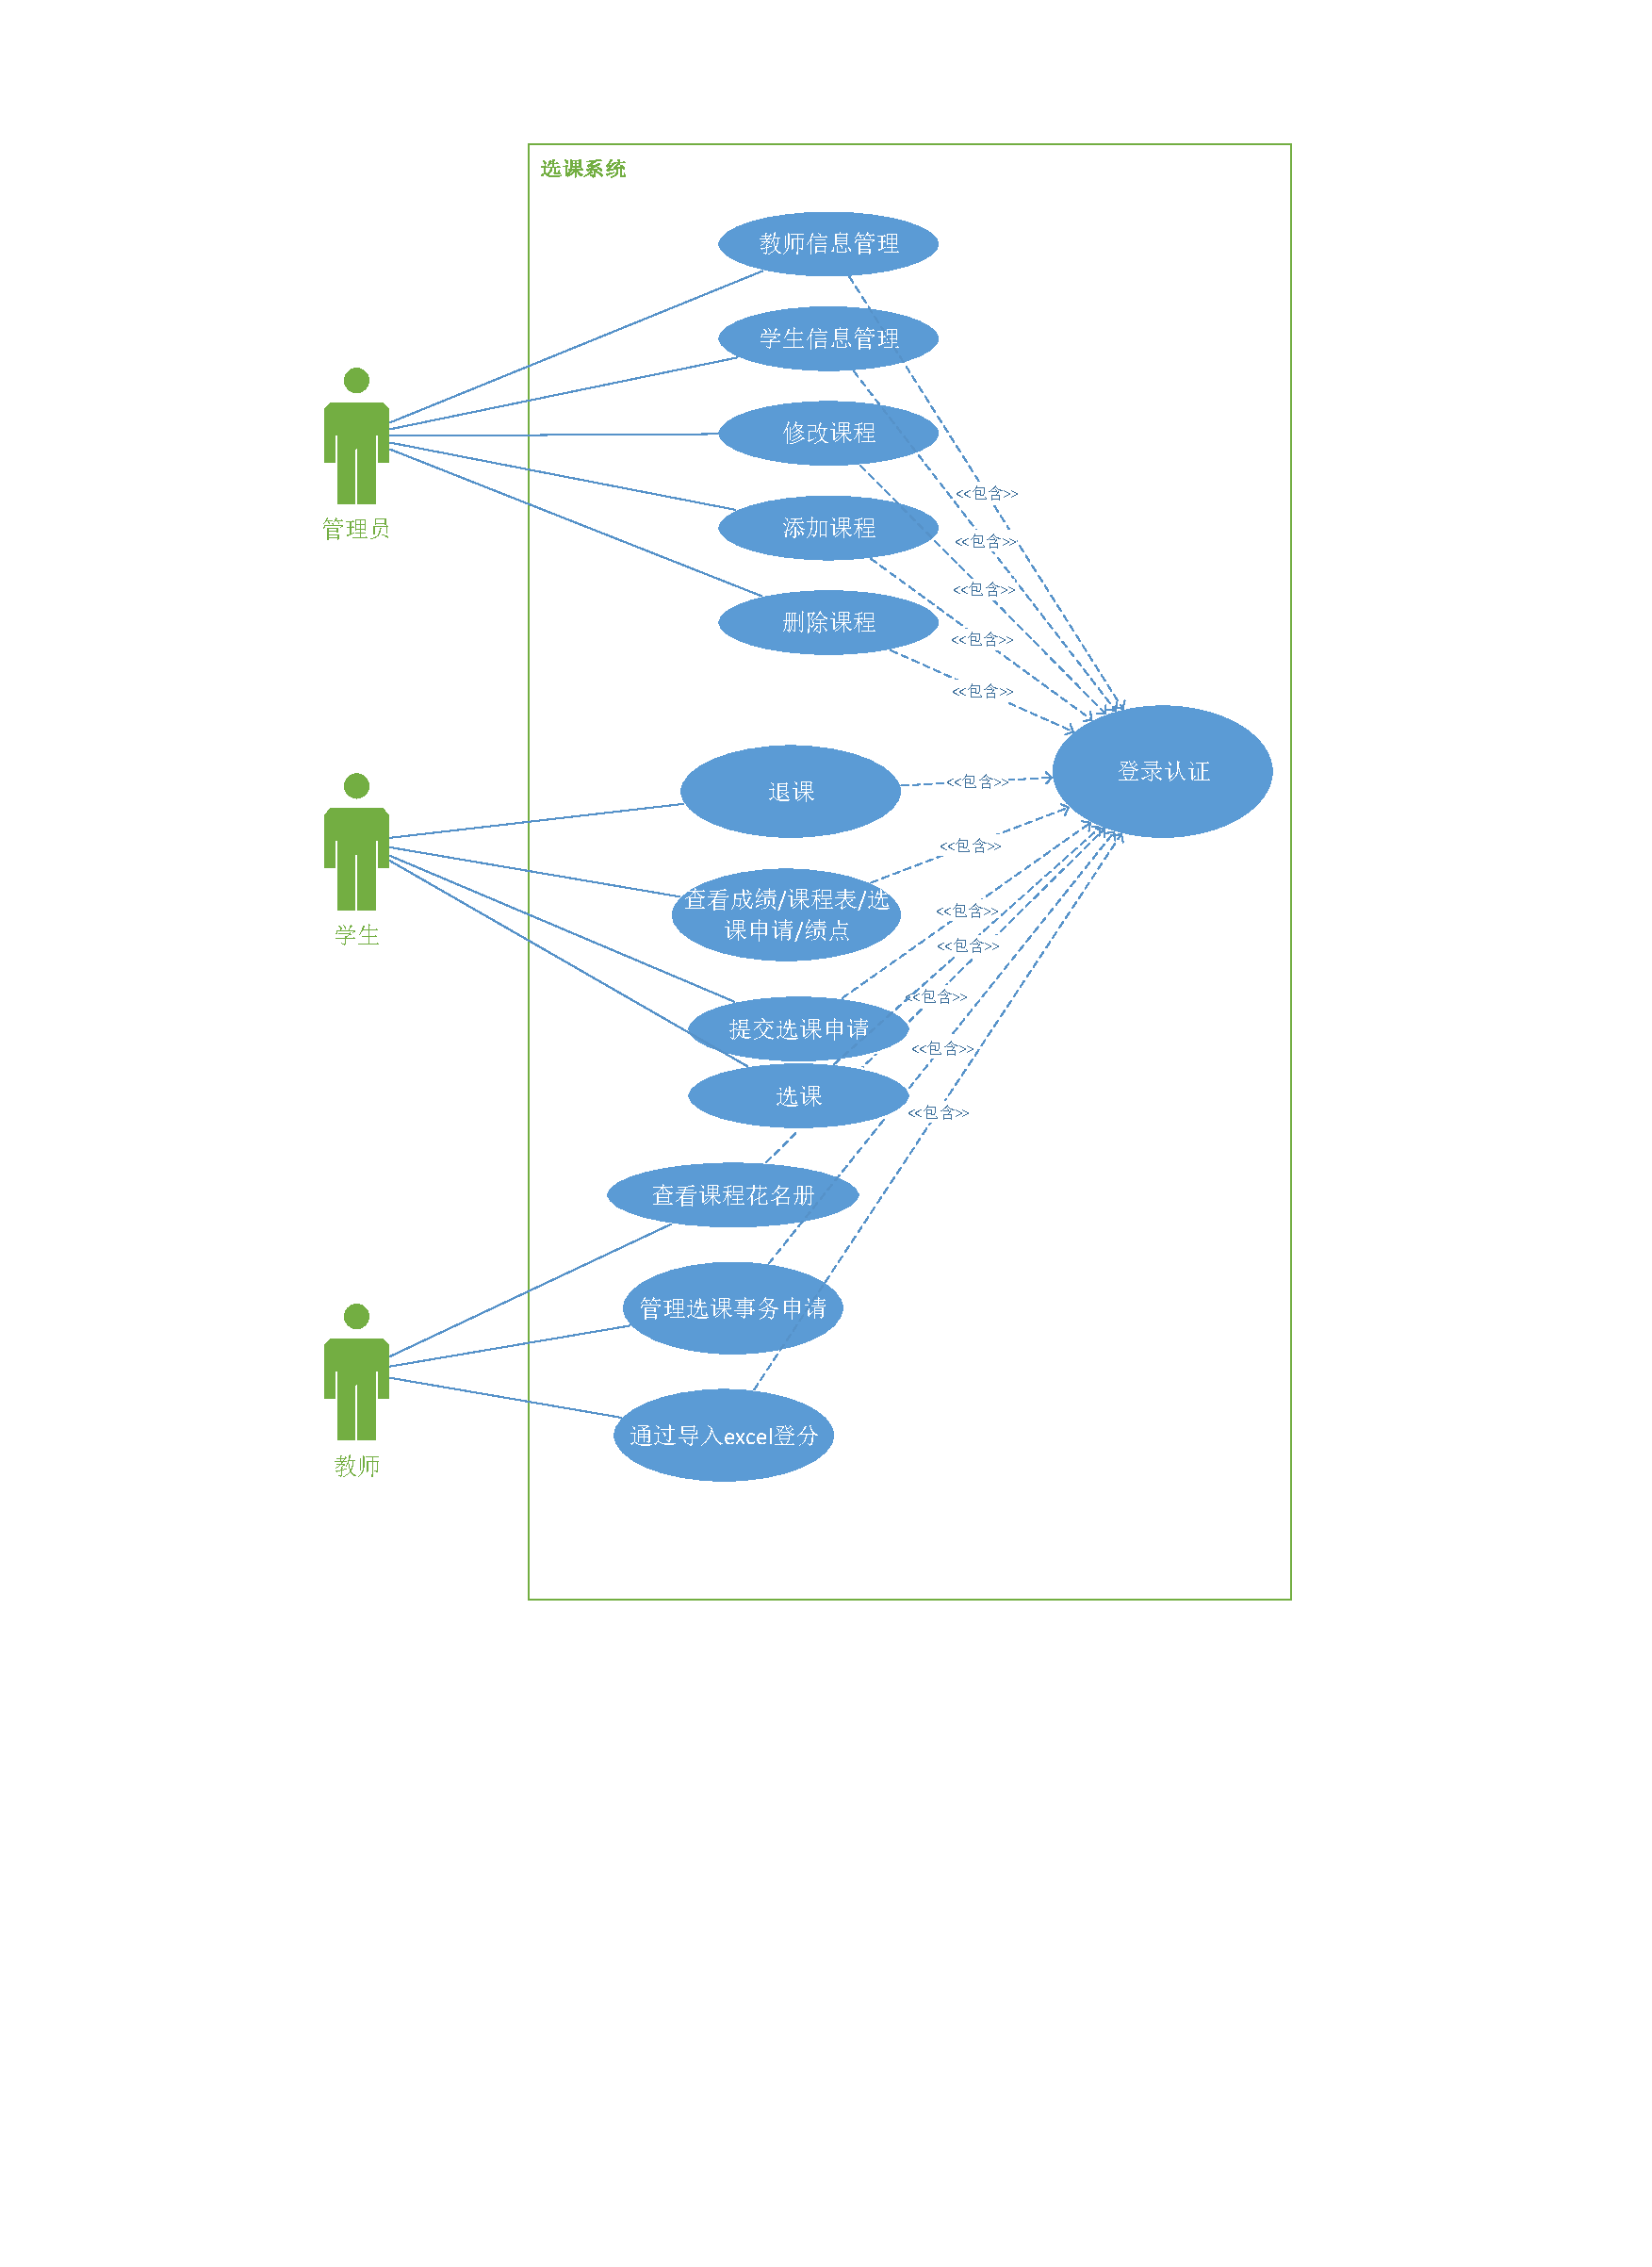
\includegraphics[width=0.8\textwidth]{assets/courseTakingusercase.pdf}
    \end{figure}

\subsection{限制检查}
\subsubsection{开设课程}
系统管理员导入或添加课程时,系统需要检查课程的相关信息是否存在冲突。检查包括但不限于:同一任课教师在多门课程的任课时间是否存在冲突;多门课程在时空上是否存在冲突;每一门课程涉及的时间和教室是否可用。系统发现冲突需要暂停执行并给出相应提示。
\subsubsection{选修课程}
学生选择课程时,系统需要检查选课的相关信息是否存在冲突。检查包括但不限于:同一学生选择的多门课程的上课时间是否存在冲突;同一学生选择的多门课程的考试时间是否存在冲突。系统发现冲突需要暂停执行并给出相应提示。
\subsubsection{选课申请}
当且仅当课程的选课人数到达上限,学生可以填写选课申请,否则,系统自动驳回。并且学生不能申请选已退课程。当学生所选课程的选课人数超出教室可容纳人数时,系统自动驳回尚未处理的选课申请,关闭该课程的申请窗口。
\subsection{测试需求}

\begin{itemize}
    \item 自动导入课程功能:在初始数据中出现冲突数据,并抛出相关提示。
    \item 选退课功能:在初始数据中出现冲突数据,并抛出相关提示。
\end{itemize}



